\section{Theory and Literature}



\subsection{Reinforcement Learning}
Machine learning is concerned with algorithms that learn from experience over time by processing information. Reinforcement learning is the branch of AI and machine learning where an intelligent agent tries to maximize its total reward by performing actions in an environment. In other words, an agent interacts with its environment and learns to adjust the environment towards preferred states. 

\begin{figure}[h]
    \centering
    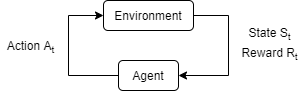
\includegraphics[width = 8cm]{Figures/RL Diagram.png}
    \caption{\centering Agent-environment interaction in reinforcement learning.}
    \label{fig: RL diagram}
\end{figure}
\noindent
An agent may like or dislike the current state of its environment. This preference is represented by a reward signal. The agent goes through a repeating sequence of states, rewards, and actions (figure \ref{fig: RL diagram}). Such a sequence from beginning to end is called a trajectory. The goal of the agent is to take actions that result in a trajectory with the highest total reward. The total reward of an entire trajectory is called the return. 


The agent chooses what actions to take based on its current state. The action strategy is called the policy '$\pi$'. The policy of an agent determines the action probability from any state. An action $A_t$ is drawn from the policy $\pi(A_t|S_t)$ of the agent. Similarly a state $S_t$ is drawn from the state-transition probability distribution $P(S_{t+1}|S_t,A_t)$ of the environment. The difference is that the state-transition dynamics do not change, while the policy is updated in an attempt to maximize the agent's return.





\subsubsection*{The Return}
The agent receives an observation of the state $S_t$ and a reward signal $R_t$ at time \textit{t}. The return is generally determined as the discounted sum of rewards in a trajectory:

\begin{equation}
    G_t = \sum_{k=t+1}^{T} \gamma^{k-(t+1)} R_k,
    \label{eq: return}
\end{equation}

\noindent
where successive returns are related to each other by:

\begin{equation}
    G_t = R_{t+1} + \gamma G_{t+1}.    
    \label{eq: return sequence}
\end{equation}
\\[-3mm]
\noindent
Equation \ref{eq: return} defines the \textit{return} as the summation over rewards multiplied by the discount factor $\gamma \in (0,1)$ from the start until termination time T. The discount factor is included to penalize distant rewards. There is no penalty when $\gamma = 1$, and only the first reward has value to the agent when $\gamma = 0$. The optimal discount factor depends on the problem, but is usually $\sim$0.99. 




\subsubsection{Value Functions}
Each state has a \textit{value} that determines how much reward the agent is expected to get from that particular state onward. It is useful to know these state values, since agents can then take actions that direct them towards higher valued states. The value of a state is defined as the expected return of that state:

\begin{equation}
    \label{eq: state value function}
    V^\pi(s) = \mathbb{E}_\pi[G_t\ |S_t = s].
\end{equation}
\\[-3mm]
\noindent
This is the \textit{state-value function} following policy $\pi$. The value of state 's' is equal to its estimated return. Another useful value function is the action-value function. This function estimates the value of a state-action pair:

\begin{equation}
    Q^\pi(s,a) = \mathbb{E}_\pi[G_t\ |S_t = s, A_t = a].
    \label{eq: action value function}
\end{equation}
\\[-3mm]
\noindent
The \textit{action-value function} following policy $\pi$ describes the expected return if the agent starts in state s, performs action a, and from there takes actions based on policy $\pi$ until termination. 
\\\\
The advantage of an action is a measure of how good the action is in a particular state. Th \textit{advantage function} can be calculated by subtracting equation \ref{eq: action value function} from equation \ref{eq: state value function} for a specific action: 
\\[-3mm]
\begin{equation}
    A^\pi(s,a) = Q^\pi(s,a) - V^\pi(s).
\end{equation}
\\[-2mm]
\noindent
The advantage function can be seen as the Q-function with lower variance since the V-value is subtracted as a baseline. If the advantage function is positive for a state-action pair, the agent expects more return in state s from performing action a than following policy $\pi$.

\subsubsection*{Optimal Policy}

If the value function following policy $\pi$ is at its maximum for all states, this policy is called optimal. There is always at least one optimal policy $\pi^*$.  If the state-value and action-value functions follow the optimal policy, these functions are by definition also optimal:
\\[-4mm]
\begin{gather}
        \label{eq: V optimal}
        V^*(s) =  \underset{\pi}{max} \, V^\pi(s), \\ 
        Q^*(s,a) =  \underset{\pi}{max} \, Q^\pi(s, a).
        \label{eq: Q optimal}
\end{gather}
\\[-2mm]
\noindent
Function \ref{eq: V optimal}  and \ref{eq: Q optimal} are the \textit{optimal state-value function} and the \textit{optimal action-value function}. These functions follow the policy that returns the highest value for each state. The optimal policy is only known in very simple problems like tic-tac-toe. In more difficult environments like chess, it becomes infeasible to find the optimal policy due to the enormous number of possible trajectories. Finding a policy as close to this optimal policy as possible is at the heart of reinforcement learning. 

\newpage

\subsubsection*{The Bellman Equations}

Approaching the real values of the value functions is an optimization problem. The Bellman equations are equations that break down this optimization problem into multiple simpler problems. There are four Bellman equations. The first Bellman equation states that the current value of a state is the reward from that state plus the value of the next state:

\begin{equation}
    \label{eq: 1st bellman equation v-policy}
    V^\pi(s) =  \underset{\underset{s' \sim P}{a' \sim \pi }}{\mathbb{E}} \ [R(s,a')\ +\ \gamma V^\pi(s')].
\end{equation}
\\
\noindent
Here, the a' and s' stand for the upcoming action and state drawn from the policy and the environment. The reward plus next value on the right side of the equation is called the \textit{Bellman backup}.

As for the state's V-value, there is also a Bellman equation for the state-action Q-value. Similar to the previous equation \ref{eq: 1st bellman equation v-policy}, this Bellman equation finds its value by the current reward plus the value of the next state-action pair:

\begin{equation}
    \label{eq: 2st bellman equation q-policy}
    Q^\pi(s,a) =  \underset{\underset{s' \sim P}{a' \sim \pi }}{\mathbb{E}} \ [R(s,a)\ +\ \gamma Q^\pi(s',a')]
\end{equation}


\begin{equation*}
    = \underset{a}{\sum}  \pi(a|s) \underset{s'}{\sum} P(s'|s,a) \ 
    [R(s,a)\ +\ \gamma Q^\pi(s',a')].
\end{equation*}
\\
\noindent
This equation is expanded to find the meaning of the expectation $\mathbb{E}$. The expectation averages all possibilities weighted by the probability of occurring. In the case of equation \ref{eq: 2st bellman equation q-policy}, the Q-value is estimated as a weighed sum over the possible actions and states multiplied by the Bellman backup. These actions a' and states s' are given by the policy and the state-transition distributions. Both these distributions sum up to one, since each time-step includes one action and one state.

The final two Bellman equations are the optimal versions of equation \ref{eq: 1st bellman equation v-policy} and \ref{eq: 2st bellman equation q-policy}. They are similar to the previous equations, except for the choice of the upcoming action a'. Instead of summing over each possible action in the policy, an optimal action is selected.



\begin{gather}
    \label{eq: 3rd bellman equation v-optimal}
    V^*(s) = \underset{a'}{max} \underset{s' \sim P}{\mathbb{E}} \ [R(s,a')\ +\ \gamma V^*(s')], \\ 
    Q^*(s,a) =  \underset{s' \sim P}{\mathbb{E}} \ [R(s,a)\ +\ \gamma \, \underset{a'}{max} \, Q^*(s',a')].
    \label{eq: 4rd bellman equation q-optimal}
\end{gather}
\\[-2mm]
\noindent
In these optimal Bellman equations, the action a' is chosen such that the return is maximized. In a solved optimization problem, the V*-values and Q*-values are the true state and action values. In this case, an optimal policy always takes an action that obeys:

\begin{equation}
    A^* = arg\, \underset{a}{max} \, Q^*(s,a).
\end{equation}


\newpage












\subsubsection{Learning from Interaction}

In reinforcement learning, there are two main methods to learn the state and action value functions from interaction with an environment. These are the Monte Carlo and Temporal Difference methods. 

\subsubsection*{Monte Carlo}

\textit{Monte Carlo} (MC) is a class of learning methods where the values are updated only after an entire episode is generated. Each episode is a trajectory of state-action-reward time-step from start to finish. This trajectory is sampled from the probability distributions of the environment's dynamics and the agent's policy. After an episode is generated, the return at each time-step t in this episode is calculated from the final step backwards. Each value is updated by:

\begin{equation}
    \label{eq: Monte Carlo Value Update}
    V(S_t) \leftarrow V(S_t) + \alpha [G_t - V(S_t)].
\end{equation}
\\[-2mm] \noindent
The syntax of this update on the state value function $V(S_t)$ also works to update the action value function $Q(S,A)$. In the update the $[G_t - V(S_t)]$ term represents the difference between the sampled return G and the expected return V at time t. The return G is called the \textit{target}, and the value V is updated to better resemble this target. $\alpha \in (0,1)$ is the step size that determines the rate of learning. Nothing new will be learned when $\alpha = 0 $, and only the newest sample is taken into account when $\alpha = 1$. In practice, an $\alpha$ of $\approx 0.00025$ balances between these two extremes. 




\subsubsection*{Temporal Difference}

As with Monte Carlo, \textit{temporal difference} (TD) methods learn from experience without a model of the environment's dynamics. The main difference between the two methods is that temporal difference methods \textit{bootstrap}. With bootstrapping the value estimates are updated with the use of other value estimates. This makes it possible to update the value function without the need to finish an entire episode:

\begin{equation}
    V(S_t) \leftarrow V(S_t) + \alpha [(R_{t+1} + \gamma V(S_{t+1})) - V(S_t)].
\end{equation}
\\[-2mm] \noindent
The value of a state is updated by only using the next reward $R_{t+1}$ and next state value $V(S_{t+1})$. The values can thus be updated directly after each step. The target $(R_{t+1} + \gamma V(S_{t+1}))$ is motivated by the Bellman backup of equation \ref{eq: 1st bellman equation v-policy}. The value is updated a step $\alpha$ in the direction of this target. 

A Monte Carlo trajectory produces an unbiased estimation of the value of each visited state, since the actual return is used as a target. However, due to the broad range of possible trajectories the variance of the return is high. In contrast, temporal difference include a bias, since the values are based on other value estimations and not solely on observations. However, bootstrapping has a lower variance as an advantage. 

The two main TD methods are Sarsa and Q-learning. The difference between these two methods is that Sarsa learns on-policy, and Q-learning learns off-policy. An explanation on this difference is given after the reinforcement learning problem is explained. % (\ref{eq: SARSA update} and \ref{eq: Q-learning update}).


\subsubsection*{Prediction and Control}

% Prediction
The reinforcement learning problem can be split into a prediction and a control problem. In the \textit{prediction problem} the state values are estimated based on the current policy. In the \textit{control problem} the policy is updated to better suit the latest estimated values. The value and policy are repeatedly updated in succession with respect to each other. In theory, this iterative interaction of prediction and control converges to a global optimum. However, in practice the process does not always converge or gets stuck in a local optimum. This instability can have multiple reasons like insufficient data, improper hyperparameters, or a learning method that is unfit for the problem. Moreover, the agent needs to properly balance exploration with exploitation to approach a global optimum. 

\subsubsection*{Exploration and Exploitation}

With \textit{exploitation} the agent chooses actions that are expected to return the highest reward. Exploitation is needed to increase data on the most promising states and actions. By only exploiting, trajectories that initially show little return are not further explored. This makes it possible to get trapped in a local optimum. The policy of an agent should therefore also include \textit{exploration}. For example, the $\epsilon$-greedy policy chooses an action at random with probability $\epsilon$, and otherwise acts to maximize expected return.

\subsubsection*{On-Policy and Off-Policy}
The value function can be learned on-policy and off-policy. Both these learning methods balance exploration with exploitation differently. With \textit{on-policy} learning, the actions are sampled from the same policy that is optimized. With \textit{off-policy} learning, the learned behavior does not necessarily reflect the agent's actions. Off-policy methods use two separate policies, the target policy and the behavior policy. The goal in off-policy learning is to optimize for the \textit{target policy} while taking actions from the \textit{behavior policy}. Due to this separation between the two policies, off-policy methods are more general. Off-policy learning enables \textit{experience replay} where an agent learns by reviewing stored experiences. These stored experiences do not have to be from the learning agent itself.




\subsubsection*{Sarsa}
\textit{Sarsa} is the most basic on-policy, temporal difference, control method. Because Sarsa is a control method the action value function $Q(S,A)$ is used instead of the state value function $V(S,A)$: 

\begin{equation}     \label{eq: SARSA update}
    Q(S_t, A_t) \leftarrow Q(S_t, A_t) + \alpha [(R_{t+1} + \gamma Q(S_{t+1}, A_{t+1}))  - Q(S_t, A_t) ].
\end{equation}
\\[-2mm] \noindent
The next action $A_{t+1}$ is sampled from the policy. This makes the action value update  on-policy. For example, an $\epsilon$-greedy policy chooses the action $A_{t+1}$ to maximize the value $Q(S_{t+1}, A_{t+1})$ with chance ($ 1-\epsilon$), or at random with chance $\epsilon$.

The next value $Q(S_{t+1}, A_{t+1})$ can itself be split up into into an upcoming reward and discounted value $R_{t+2} + \gamma Q(S_{t+2}, A_{t+2})$ to get a nested update of the action value. This technique of nested updates is called \textit{n-step bootstrapping}, where the temporal difference extends over the amount of nested steps n. If the steps are updated all the way through the end of the sample trajectory, the TD method becomes a Monte Carlo method.  










\subsubsection*{Q-Learning}

As with Sarsa, \textit{Q-learning} is a temporal difference, control method. The difference is that Q-learning is off-policy.  The target in the Sarsa update contains the action value $Q(S_{t+1}, A_{t+1})$ where the action that determines this action value is chosen by the policy. In contrast, the action in the target of Q-learning is chosen to maximize the action value:

\begin{equation}    \label{eq: Q-Learning update}
    Q(S_t, A_t) \leftarrow Q(S_t, A_t) + \alpha [(R_{t+1} + \gamma \, \underset{a}{max} \, Q(S_{t+1}, a))  - Q(S_t, A_t) ].
\end{equation}
\\[-2mm] \noindent
In this update the action \textit{a} that maximizes the value $Q(S_{t+1}, a)) $ is chosen to bootstrap the action value from. The behavior policy does not have an effect on this update, since the update always chooses the optimal action value regardless of the policy. This makes Q-learning off-policy.



% \subsubsection{Planning with Models}

% Some reinforcement learning methods improve solely from experience on the actual environment. These are called \textit{model-free} methods. Other methods require a model of the environment to operate, either to learn or to plan ahead. These are called \textit{model-based} methods. 

% planning versus learning, model

% Given vs learned model

% planning at decision time (MCTS)

% dynamic programming










\subsubsection{Neural Networks}

% 1. Why function approximation

In basic \textit{tabular methods} each value is stored individually. In many reinforcement learning problems however, the number of possible states of an environment vastly exceeds the number of computer bits. It is impossible to keep track of every value individually, due to the memory needed to store these values, and the time to get samples from each state. Luckily, the values can be approximated by generalizing between similar states. This generalizing is often done with the use of \textit{Artificial Neural Networks} (ANNs). An ANN takes for example a state as input and can generalize this state to similar observed states as a way to estimate the state's value. These networks are inspired by the structure of neurons inside a biological brain.

\subsubsection*{Feedforward Neural Networks}

An Artificial Neural Networks is a \textit{non-linear function approximator}. ANNs can approximate any function depending on the structure of the ANN. An ANN is made up of multiple \textit{nodes} that are connected with \textit{edges}. A \textit{feedforward neural network} is a network where the nodes in each layer are connected to nodes in the next layer. The first and last layers are the input and output layers, and the layers in the middle are the \textit{hidden layers}. 


With \textit{fully connected} (dense) layers, each node is connected to every node in the previous layer. According to the universal approximation theorem, one hidden dense layer with an arbitrary number of nodes is enough to approximate any function.


%Another type of widely used NN is the convolutional neural networks (CNN). This class of NN is able to analyze images by looking at several levels of abstraction, by means of convolution and subsampling. 





\subsubsection*{Neurons}

Each node in a neural network acts as a simple individual function through which signals are passed:

\begin{equation}
    y_m = f( \underset{n}{\sum} \theta_{mn} x_n )
\end{equation}
\\[-2mm] \noindent
In this function, the node \textit{m} receives the output of other nodes $x_n$ as input. The input values are multiplied by the \textit{weights} $\theta_{mn}$ of the edges that connect each input node to node m. The weighted value of each input node is summed together. This resulting summation is inserted in the function \textit{f} to produce the output $y_m$ of node \textit{m}. 

The function \textit{f} is the \textit{activation function}. This function is required to add a non-linearity into the system. The non-linearity is needed because linear functions of linear functions are also linear, which would make them unfit to approximate non-linear function. A simple example of an activation function is the rectified linear unit (ReLU): $f(x) = max(0,x)$. Other popular activation functions are the S-shaped logistic function $f(x) = 1/(1+e^{-x})$ and the hyperbolic tangent function $f(x) = tanh(x)$. 









\subsubsection*{Backpropagation}

% 4. Loss + Backpropagation 

Feedforward neural networks can be trained with the \textit{backpropagation} algorithm. With backpropagation, the weights of the neural networks are updated via \textit{stochastic gradient descent} (SGD). Gradient descent is the principle where weights are adjusted in the direction of a lower error by taking the derivative of the loss with respect to each weight. The gradient descent is called stochastic when the training data is randomly sampled. 

The loss function \textit{L} is often calculated as the squared difference between the target Y and the estimated value of the ANN:

\begin{equation}
    L(\WeightVector) = (Y - V(s;\WeightVector))^2
\end{equation}
$\WeightVector$ is the \textit{weight vector} that consists of all the weights in the ANN. Each weight can be individually adjusted to reduce the loss. This is done by taking a step $\alpha$ in the direction of steepest descent:

\begin{equation} \label{eq: individual weight update}
    \theta_{mn} = \theta_{mn} - \alpha \frac{\delta L}{\delta \theta_{mn}}
\end{equation}
This function can also be written for all weights simultaneously:


\begin{equation}
    \WeightVector = \WeightVector  - \alpha \nabla_{\theta} L
\end{equation}
The del operator $\nabla$ denotes the gradient operation. $-\nabla_{\theta} L$ points in the direction of steepest descent. The magnitude of $\nabla_{\theta} L$ is equal to the steepness of this slope. As the weight vector $\WeightVector$ is constantly updated in the direction of lower loss, the value estimations of the ANN get closer to the targets.


% Variable step size SGD: RMSProp/Adam etc

% mini-batch






% \subsubsection{Policy Gradient Methods}

% basics
% Neural network maps states to actions in the case of policy approximation.

% Policy Gradient Theorem

% REINFORCE or VPG, Monte-Carlo PG   baseline

% Actor Critic




